\documentclass{article}
\usepackage{amsfonts}

\usepackage{amsmath}
\DeclareMathOperator*{\argmax}{arg\,max}
\DeclareMathOperator*{\argmin}{arg\,min}

 
\usepackage{geometry}
 \geometry{
 a4paper,
 left=30mm,
 top=25mm,
}

\usepackage{hyperref}
\usepackage{cite}
\usepackage[utf8]{inputenc}
\usepackage{listings}
\usepackage{graphicx}
\usepackage[ruled,vlined]{algorithm2e}
\usepackage{color}
 
\definecolor{codegreen}{rgb}{0,0.6,0}
\definecolor{codegray}{rgb}{0.5,0.5,0.5}
\definecolor{codepurple}{rgb}{0.58,0,0.82}

\definecolor{backcolour}{rgb}{0.95,0.95,0.92}
\lstdefinestyle{mystyle}{
    backgroundcolor=\color{backcolour},   
    commentstyle=\color{codegreen},
    keywordstyle=\color{magenta},
    numberstyle=\tiny\color{codegray},
    stringstyle=\color{codepurple},
    basicstyle=\footnotesize,
    breakatwhitespace=false,         
    breaklines=true,                 
    captionpos=b,                    
    keepspaces=true,                 
    numbers=left,                    
    numbersep=5pt,                  
    showspaces=false,                
    showstringspaces=false,
    showtabs=false,                  
    tabsize=2
}
 
\lstset{style=mystyle}

\title{IE 613: Assignment 1}
\author{Manan Doshi \\ 140100015}
\date{20 February 2018}

\begin{document}
\graphicspath{{./plots}}
\maketitle

\section*{Question 1: FoReL and WM Equivalence}

In this question, we show that the Weighted Majority algorith we developed for the case of a finite number of experts is a special case of the FoReL algortihm when:
\begin{align*}
    R_w  &= \frac{1}{\eta}\sum_{j=1}^{d} w_j \log w_j \qquad &\text{$R_w$ is the regularizer}\\
    f_t(w) &= \langle w,v_t \rangle \qquad &\text{$f_t(w)$ is the linear loss function}\\
    \sum_{j=1}^{D} w_j &= 1 \qquad &\text{$w$ does not span the entire space $\mathbb{R}_d$}\\
\end{align*}

We show that this is analogous to the WMA with $D$ experts where $v_t$ is the loss vector associated with round $t$ and $w_t$ is the (regularized) weight of each expert.\\
For the FoReL algorithm:
\begin{align*}
    w_t &= \argmin_{w} \left( \sum_{i=1}^{t-1} f_i(w) + R(w) \right) &\qquad\\
    &= \argmin_{w} \left( \sum_{i=1}^{t-1} \langle w,v_i \rangle + \frac{1}{\eta} \sum_{j=1}^{D} w_j \log w_j \right) &\qquad \text{Substituting regularizer and loss terms}\\
\end{align*}

We need to find the optimal value of $w$ under the constraint $\sum_j w = 1$. We use the lagrange multiplier method.
\begin{align*}
    l(w) &= \left( \sum_{i=1}^{t-1} \langle w,v_i \rangle + \frac{1}{\eta} \sum_{j=1}^{D} w_j \right)\ &\qquad \text{We wish to minimise this function}\\
    c(w) &= \sum_{j=1}^{D} w_j - 1 &\qquad \text{under the constraint that $c=0$}\\
    \nabla_w(l(w)) &=\sum_{i=1}^{t-1} v_i + \frac{1}{\eta}\left( \bf{1} + \log w \right) \\
    \nabla_w(c(w)) &= \bf{1}\\
    \mathcal{L}(w) &= l(w) - \lambda c(w) \\
    \nabla_{w,\lambda}\mathcal{L}(w,\lambda) &= 0  &\qquad \text{Lagrange multiplier method}\\
    \sum_{i=1}^{t-1} v_i + \frac{1}{\eta}\left( \bf{1} + \log w \right) &= \lambda(\bf{1})
\end{align*}
Solving for $w$,
\begin{align*}
    w_t &= \exp (\eta \lambda - 1) \exp (-\eta \sum_{i=1}^{t-1}v_i)\\
    w_{j,t}    &= \frac{e^{-\eta \sum_{i=1}^{t-1}v_{i,j}}}{\sum_{j=1}^{D}e^{-\eta \sum_{i=1}^{t-1}v_{i,j}}} &\qquad \text{This is because we choose $\lambda$ such that the constraint is satisfied}\\
\end{align*}

This is the exact same expression obtained in WMA, where $v_{i,j}$ in the loss suffered by Expert $j$ in round $i$. The $\eta$ here is the same as the $\eta$ in WMA. The optimal $\eta$ will thus be

\[
    \eta^* = \sqrt{\frac{2 \log D}{T}}
    \]

\newpage
\section*{Question 2: Online Convex Optimisation}
Following are the plots generated by running the FTL and FoReL algorithms on the given systems. Averages are taken over $30$ paths and the $95\%$ confidence interval is shown using the shaded region. Code for this question can by found \href{run:./code/Q2_3.py}{here} 

\begin{figure}[h!]
\centering
\includegraphics[scale=0.3]{q2}
\caption{Expected regret as a function of times for FTL and FoReL algorithms working on the given system}
\end{figure}

It can be clearly seen that the confidence interval of FoReL is tighter. This is due to the stabilising effect of the regularisation term.

\newpage
\section*{Question 3}

Below is the variation of the final expected regret for the FoReL algorithm with varying regularization coefficient. The obtained plot is pretty much the same as the one obtained for WMA.
\begin{figure}[h!]
\centering
\includegraphics[scale=0.5]{q3}
\caption{Variation of expected regret with $\eta$ for the FoReL algorithm}
\end{figure}

\newpage
\section*{Question 4: Online Classifier}
A bias term was first to the feature set. The Perceptron algorithm was applied as-is. Since the Winnow algorithm requires the equation of the seperationg plane to have positive coefficients, the feature set was modified based on the weights obtained by the perceptron algorithm. The feature set was also shifted to make the seperating plane obtained by the perceptron algorithm to pass through the origin. The winnow algorithm was then applied to this modified dataset. Below are the results obtained.
\begin{figure}[h!]
\centering
\includegraphics[scale=0.3]{skin}
\caption{Performance on the two algorithms on the Skin Segmentation Dataset}
\end{figure}

\begin{figure}[h!]
\centering
\includegraphics[scale=0.3]{wine}
\caption{Performance on the two algorithms on the Wine Quality Dataset}
\end{figure}

\begin{figure}[t!]
\centering
\includegraphics[scale=0.3]{news}
\caption{Performance on the two algorithms on the Online News Popularity Dataset}
\end{figure}

\clearpage
\section*{Question 6}
Following are the seperating planes generated by the two algorithms for the same dataset
\begin{figure}[h!]
\centering
\includegraphics[scale=0.3]{q6a}
\caption{Performance on the two algorithms on the generated Dataset}
\end{figure}

An estimate of the margin is computed by creating multiple datasets and computing the margin for that dataset assuming the optimal seperating plane is parallel to $x+y+12=0$. The estimated margin comes out to be $3.97$. Similarly, the estimated value for the max norm comes out to be $16.11$. Using this numbers, the Mistake bound for the perceptron algorithm is
\begin{align*}
    M &\leq \left(\frac{R}{\gamma}\right)^2\\
    &=\left(\frac{16.11}{4.11}\right)^2\\
    M &\leq 16\\
\end{align*}
This is obeyed in our simulation.\\

Next we see the variation of the number of mistakes made ny the winnow algorithm as a function of the learning rate (with a 95\% confidence interval. The system is regenerated and multiple runs are done). When the learning rate is very low, a high number of mistakes are made. This is expected since the classifier is very slow to respond to data. When the learning rate is very high, the confidence interval widens. The algorithm starts making more mistakes as it overshoots everytime there is a mistake.
\begin{figure}[h!]
\centering
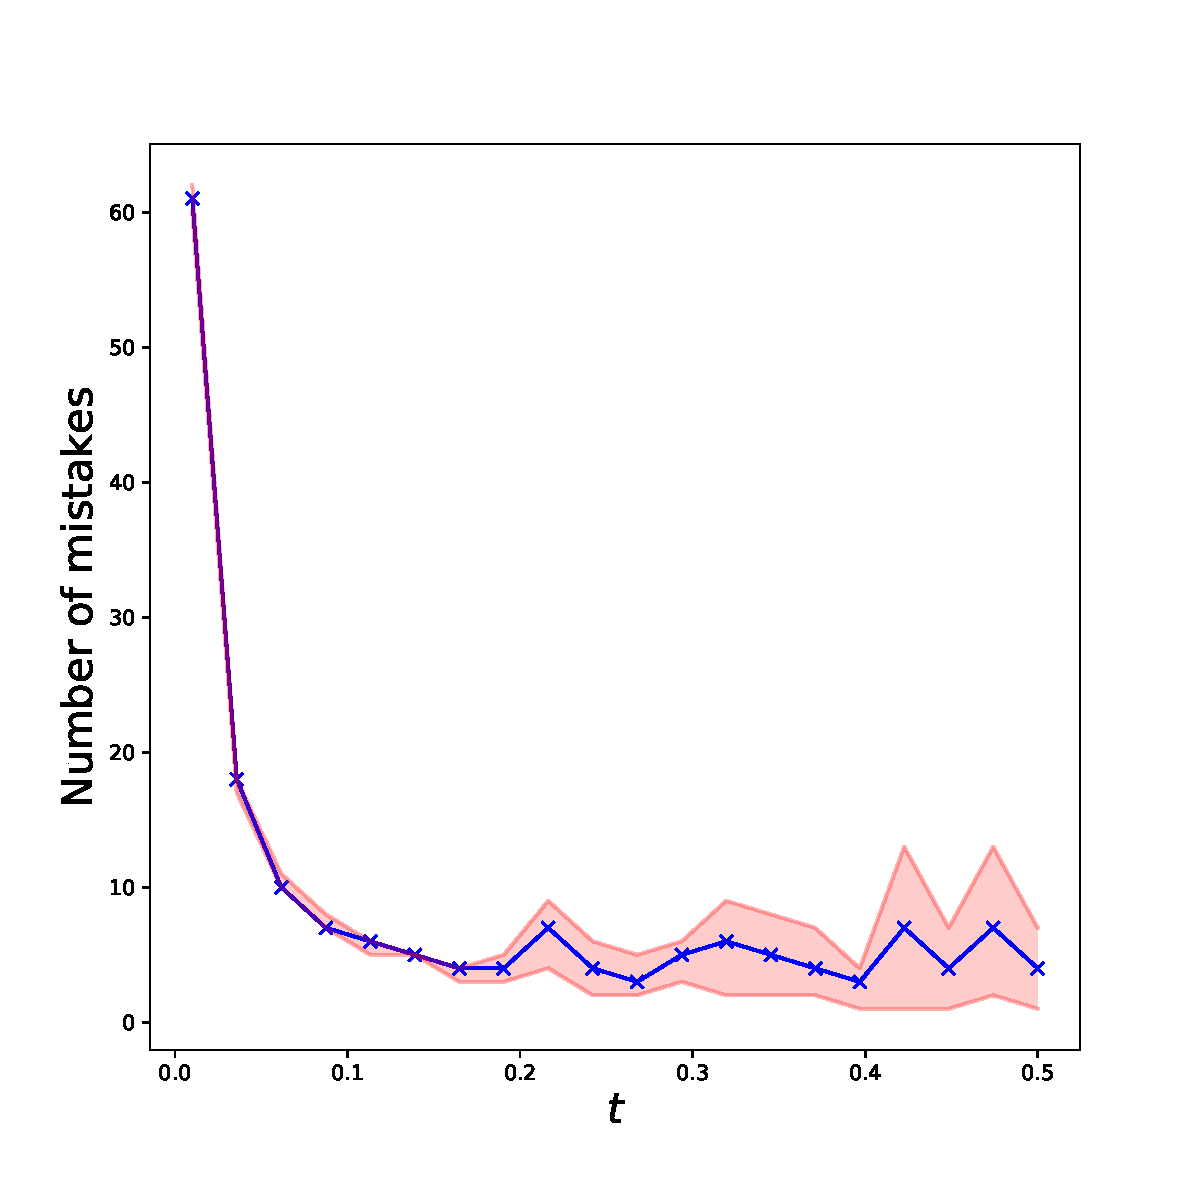
\includegraphics[scale=0.4]{q6b}
\caption{Performance of the winnow algorithm with various learning rates}
\end{figure}
\clearpage
\section*{Question 7}
We compare the performance of OGD and OMD. OGD behaves as expected, making a lot of errors initially. The regret finally flattens out, implying that the algorithm is correct on most of the new data. The implementation of OMD is possibly incorrect. The 95\% confidence intervals are plotted by doing multiple runs where a new dataset is generated and shuffled everytime.
\begin{figure}[h!]
\centering
\includegraphics[scale=0.3]{q7}
\caption{Performance of the OGD and OMD algorithms}
\end{figure}
%
%\newpage
%
%\section*{Question 2}
%\subsection*{Code}
%\subsubsection*{EXP3}
%\begin{lstlisting}[language=python]
%def exp3(d,T,eta):
%    e_loss = 0
%    elv = 0.5*np.ones([d,2])
%    elv[-2,:] = 0.4
%    elv[-1,:] = [0.6,0.3]
%    w_tilde = np.ones([d])
%    
%    for t in range(T):
%        w = w_tilde/np.sum(w_tilde)
%        adv_choice = np.random.choice(d,p=w)
%        e_loss_c   = elv[adv_choice,(2*t)//T]
%        l          = np.random.choice(2,\
%                     p=[1-e_loss_c, e_loss_c])/w[adv_choice]
%        e_loss    += e_loss_c
%        w_tilde[adv_choice]    = w_tilde[adv_choice]*np.exp(-eta*l)
%
%    return e_loss - 0.4*T
%\end{lstlisting}
%\subsubsection*{EXP3.P}
%\begin{lstlisting}[language=python]
%def exp3p(d,T,eta,beta,gamma):
%    e_gain = 0
%    elv = 0.5*np.ones([d,2])
%    elv[-2,:] = 0.4
%    elv[-1,:] = [0.6,0.3]
%    egv = 1-elv
%    G = np.zeros([d])
%    w_tilde = np.ones([d])
%
%    for t in range(T):
%        w                 = (1-gamma)*(w_tilde/np.sum(w_tilde)) + gamma/d
%        adv_choice        = np.random.choice(d,p=w)
%        e_gain_c          = egv[adv_choice,(2*t)//T]
%        gain              = beta/w
%        gain[adv_choice] += np.random.choice(2,\
%                            p=[1-e_gain_c, e_gain_c])/w[adv_choice]
%        e_gain           += e_gain_c
%        w_tilde           = w_tilde*np.exp(eta*gain)
%
%    return 0.6*T - e_gain
%\end{lstlisting}
%\newpage
%\subsubsection*{EXP3-IX}
%\begin{lstlisting}[language=python]
%def exp3ix(d,T,eta,gamma):
%    e_loss = 0
%    elv = 0.5*np.ones([d,2])
%    elv[-2,:] = 0.4
%    elv[-1,:] = [0.6,0.3] 
%    w_tilde = np.ones([d])
%
%    for t in range(T):
%        w = w_tilde/np.sum(w_tilde)
%        adv_choice = np.random.choice(d,p=w)
%        e_loss_c   = elv[adv_choice,(2*t)//T]
%        l          = np.random.choice(2,\
%                     p=[1-e_loss_c, e_loss_c])/(w[adv_choice]+gamma)
%        e_loss    += e_loss_c
%        w_tilde[adv_choice]    = w_tilde[adv_choice]*np.exp(-eta*l)
%
%    return e_loss - 0.4*T
%\end{lstlisting}
%\subsection*{Plot}
%\begin{figure}[h!]
%\centering
%\includegraphics[scale=0.24]{Q2}
%\caption{Variation of expected regret with $\eta$ multiplier}
%\end{figure}
%\newpage
%\section*{Question 3}
%Clearly, \verb|EXP3-IX| has the best performance with lower expected regret and lower deviation. The good performance of \verb|EXP3-IX| can be attributed to the fact that it explores and detects the new best advisor after the change in odds at $\frac{T}{2}$. This exploration is not possible in \verb|EXP3|. The bad performance of \verb|EXP3.P| can be attributed to very high exploration rates leading to low exploitation of the current best adviser. This behavious can be clearly seen in the following plot
%
%\begin{figure}[h!]
%\centering
%\includegraphics[scale=0.3]{Q3}
%    \caption{Probability contours with advisors and time for \texttt{EXP3}, \texttt{EXP3.P} and \texttt{EXP3-IX} respectively. The weak exploitation of \texttt{EXP3.P} and the slow switching of \texttt{EXP3} is apparent here.}
%\end{figure}
%\newpage
%\section*{Question 4 \cite{ben2009agnostic}}
%The proposed algorithm is the same as the wighted majority algorithm
%
%\begin{algorithm}
%    \SetKwInOut{Input}{Input}
%    \SetKwInOut{Parameter}{Parameter}
%    \SetKwInOut{init}{Initialize}
%
%    \Input{Hypothesis class $\mathcal{H}$}
%    \Parameter{$\eta \in [0,1]$}
%    \init{$\tilde{w}^{(1)} = [1, 1, 1, ... ,1]$ in \(\mathbb{R}^d\)}
%    \For{$t\leftarrow 1$ \KwTo $T$}{
%        Set $w_i^{(t)} = \frac{\tilde{w}_i^{(t)}}{\sum_i \tilde{w}_i^{(t)}}$ \\
%        Play $i$ according to the distribution $w^{(t)}$ \\
%        Receive loss vector $l_t = \{l_{t,i} :\forall i \in d\}$ where $l_{t,i}$ is the error in prediction of hypthesis $h_i$\\
%        Update $\forall i, \tilde{w}_i^{(t+1)} = \tilde{w}_i^{(t)}e^{-\eta l_{t,i}}$\\
%    }
%    \caption{The Weighted Majority Algorithm}
%\end{algorithm}
%
%We will compute a finite bound for expected number of mistakes of this algorithm on a realizable case with Bernoulli noise.
%We first make the claim that
%\begin{equation}
%\label{main}
%\mathbb{E}\left[\sum_{s=t+1}^{T}\|\hat{y}_s-f_i^s\|\right]_{w_t} \leq C_{\gamma} \ln\left(\frac{Z_t}{w_i^t}\right)
%\end{equation}
%where $i$ refers to the `correct' hypothesis. $Z_t = \sum_{i=1}^d w_i^t$ and \(C_{\gamma} = \frac{1}{1-2\sqrt{\gamma(1-\gamma)}}\).
%
%	We will now prove the above claim using induction. The base case at $t=T$ is trivial since the LHS is $0$ and the right side is positive (since $Z_t \geq w_i^t$). We will now split our hypothesis class into two groups based on whether the hypothesis classifies the round at $t$ correctly.
%\[
%	u = \sum_{j, f_j^t = f_i^t} w_j^{t-1} \qquad\qquad  \qquad v = \sum_{j, f_j^t /neq f_i^t} w_j^{t-1}
%\]
%
%$u$ is thus the total weight of the correct classifiers for the round and $v$ is the total weight of the incorrect classifiers. Probability that the algorithm classifies incorrectly is thus $\frac{v}{Z_t-1}$. There is also a chance that the system sends incorrect feedback, say with probability $p \leq \gamma$. If the feedback is incorrect the weight update is $Z_t = e^{-\eta}u+v$ and the update of the weight of the correct hypothesis class is $ w_i^t = e^{\eta} w_i^{t-1} $. If the system send correct feedback (with probability \(1-p\)) and the weight of the correct hypothesis remains unchanged. Expected mistakes from $t$ to $T$ equals the expected number of mistakes at $t$ plus the expected number of mistakes from $t+1$ to $T$. This leads us to
%\begin{align*}
%	\mathbb{E}\left[\sum_{s=t}^{T}\|\hat{y}_s-f_i^s\|\right]_{w_{t-1}} &= \mathbb{E}\left[\sum_{s=t+1}^{T}\|\hat{y}_s-f_i^s\|\right]_{w_t} + \frac{v}{Z_{t-1}} \\
%&\leq \frac{v}{Z_{t-1}} + \mathbb{E}\left[C_{\gamma}\ln{\left(\frac{Z_t}{w_i^t}\right)}\right]_{w_t}\\
%&= \frac{v}{Z_{t-1}} + p\left[C_{\gamma}\ln{\left(\frac{e^{-\eta}u + v}{e^{-\eta}w_i^{t-1}}\right)}\right] +  (1-p)\left[C_{\gamma}\ln{\left(\frac{u + e^{-\eta}v}{w_i^{t-1}}\right)}\right]\\
%\end{align*}
%
%We will show that the last expression is bounded by the RHS of \eqref{main}. This involves mathematical manipulations given in the appendix of \cite{ben2009agnostic}. Once we have proved \eqref{main} we can substitute $t=0$ to get an upper bound for expectation of number of mistakes.
%
%\[
%\boxed{\mathbb{E}\left[\sum_{s=1}^{T}\|\hat{y}_s-f_i^s\|\right]_{w_t} \leq C_{\gamma} \ln(d)}
%\]
%\newpage
%\section*{Question 5}
%Consider an algorithm \texttt{A} whose regret bound for $T$ rounds is $\alpha \sqrt{T}$. For $2^m$ rounds, the regret bound will be $\alpha \sqrt{2^m}$. Since we do not know the time horizon, we break the time period into pieces of size $2^m$ where $m = 0, 1, 2, \cdots$. We choose the parameter $\eta$ in terms of these smaller time periods for every packet.
%
%If the total time horizon is $T$ and the total number of `packets' is $k$,
%\begin{align*}
%    \sum_{m=0}^{k-1} 2^m +1              &&\leq T \leq &&\sum_{m=0}^{k} 2^m \\
%    1 + 1 + 2 + 2^2 + 2^3 \cdots + 2^k   &&\leq T \leq &&1 + 2 + 2^2 + 2^3 \cdots + 2^k\\
%    2^k                                  &&\leq T \leq &&(2^{k+1}-1)
%\end{align*}
%
%For a time period of $2^m$, regret is $\alpha 2^{\frac{m}{2}}$. Total regret:
%\begin{align*}
%    \mathcal{R} &\leq \sum_{m=0}^{k} \alpha 2^{\frac{m}{2}}\\
%                &\leq \alpha \left(1 + \sqrt{2} + \sqrt{2}^2 + \cdots + \sqrt{2}^k \right) \\
%                &\leq \alpha \left( \frac{2^{\frac{k+1}{2}} - 1}{\sqrt{2}-1}\right)\\
%                &\leq \alpha \left( \frac{\sqrt{2T} - 1}{\sqrt{2}-1}\right)\\
%                &\leq \alpha \left( \frac{\sqrt{2T}}{\sqrt{2}-1}\right)
%\end{align*}
%\[
%    \boxed{\mathcal{R} \leq \left(\frac{\sqrt{T}}{\sqrt{2}-1}\right) \alpha \sqrt{T}}
%\]
%
%\bibliographystyle{unsrt}
%\bibliography{ref}
\end{document}
